%%%%%%%%%%%%%%%%%%%%%%%%%%%%%%%%%%%%%%%%%%%%%%%%%%%%%%%%%%%%%%%%%%%%%%%%%%%%%%%%
%2345678901234567890123456789012345678901234567890123456789012345678901234567890
%        1         2         3         4         5         6         7         8

\documentclass[letterpaper, 10 pt, conferences]{IEEEconf}  % Comment this line out
                                                          % if you need a4paper
%\documentclass[a4paper, 10pt, conference]{ieeeconf}      % Use this line for a4
                                                          % paper
\usepackage[top = 0.75in, left = 0.75in, right = 0.75in, bottom = 0.75in]{geometry}
\IEEEoverridecommandlockouts                              % This command is only
                                                          % needed if you want to
                                                          % use the \thanks command
\overrideIEEEmargins
% See the \addtolength command later in the file to balance the column lengths
% on the last page of the document
%

% The following packages can be found on http:\\www.ctan.org
\usepackage{graphicx}
\usepackage[utf8]{inputenc}
\usepackage[T1]{fontenc}
\usepackage[polutonikogreek,english]{babel}
\usepackage{fixltx2e}
\usepackage{gensymb}
\usepackage{mathtools}
\usepackage{units}
\usepackage{amssymb}
\usepackage{amsmath}
\usepackage{algorithm}
\usepackage[noend]{algpseudocode}
%\usepackage[font=small]{caption}
%\usepackage{caption}
%\usepackage{subcaption}
%\usepackage{booktabs}

\DeclareMathOperator*{\argmin}{\arg\!\min}
\DeclarePairedDelimiter\abs{\lvert}{\rvert}%
\DeclarePairedDelimiter\norm{\lVert}{\rVert}
\newcommand{\greek}[1]{{\selectlanguage{polutonikogreek}#1}}
\newcommand\scalemath[2]{\scalebox{#1}{\mbox{\ensuremath{\displaystyle #2}}}}
\renewcommand{\vec}[1]{\mathbf{#1}}
\hyphenation{op-tical net-works semi-conduc-tor}

\title{\LARGE\bf Model Predictive Control for Underwater Robots in Ocean Waves}

\author{Daniel Fernández and Geoffrey A. Hollinger
\thanks{This work was developed for the NNMREC ALFA Project and is supported by Department of Energy grant DE-EE-0006816.0000.}
\thanks{D. Fernández, G. A. Hollinger are currently with the Robotics Program at the School of Mechanical, Industrial and Manufacturing Engineering, Oregon State University, Corvallis, Oregon, 97331-6001, United States {\tt\small\{fernanda, geoff.hollinger\}@oregonstate.edu} }
}


\bstctlcite{IEEEexample:BSTcontrol}

\begin{document}
% make the title area
\maketitle
\thispagestyle{empty}
\pagestyle{empty}

\begin{abstract}
%\boldmath
\textbf{Underwater robots beneath ocean waves can benefit from feedforward control to reduce position error. This paper proposes a method using Model Predictive Control (MPC) to predict and counteract future disturbances from an ocean wave field. The MPC state estimator employs a Linear Wave Theory (LWT) solver to approximate the component fluid dynamics under a wave field. Wave data from deployed ocean buoys is used to construct the simulated wave field. The MPC state estimator is used to optimize a set of control actions by gradient descent along a prediction horizon. The optimized control input minimizes a global cost function, the squared distance from the target state. The robot then carries out the optimized trajectory with an emphasis on real-time execution. Several prediction horizons are compared, with a horizon of \unit[0.8]{seconds} selected as having a good balance of low error and fast computation. The controller with the chosen prediction horizon is simulated and found to show a \unit[74]{\%} reduction in position error over traditional feedback control. Additional simulations are run where the MPC takes in noisy measurements of the wave field parameters. The MPC algorithm is shown to be resistant to sensor noise, showing a mean position error \unit[44]{\%} lower than the noise-free feedback control case.}
\end{abstract}

%\begin{IEEEkeywords}	
%TBD, marine robotics, wave energy, autonomous path planning, perception, oceanographic monitoring, SLAM, AUV, ROV
%\end{IEEEkeywords}

\section{Introduction} 
\label{sec:introduction}

The coastal ocean is bounded by the shoreline and the \unit[200]{m} isobath, and is a common experimental setting for field robotics. This is the most biologically productive area of ocean \cite{phillips} and is subject to the majority of natural and industrial disasters. Its proximity to the shore and coastal communities adds to a variety of economic, military, and energy research areas under development. The increased demand for robotic advancement in all of these coastal research areas predicates the need to better understand the dynamics of this environment.

Wave forces in the intermediate depths of the coastal ocean will displace a robot throughout the majority of the water column. These forces decay exponentially from the water surface as shown in Fig.~\ref{fig:flowFig}, and sufficient depths yield negligible disturbances \cite{D&D}. Because of this decay, as well as their cyclic nature, wave forces are often neglected in robotic path planning. In field applications where there is a low operational depth, a persistent wave climate, and strict localization constraints, this assumption can quickly break down. As a result, increased sensor drift can hinder the quality of robotic observations, such as those needed to close SLAM loops in \cite{kim} and \cite{chaves}.
 
Traditional PID control techniques can be used to counter wave displacements, but reaction times for underwater robots are slow relative to the changing wave forces. Given the periodicity of waves, feedforward techniques should be explored. This paper outlines how Model Predictive Control (MPC) can reduce an underwater robot's position error when station-keeping under the influence of ocean waves. A wave field is decomposed to component velocities and used as input to the model. Using this model, an optimized control input is calculated over the desired time horizon. This optimized control is shown to resist wave displacement by using thruster force to counter impending disturbances.

\begin{figure}
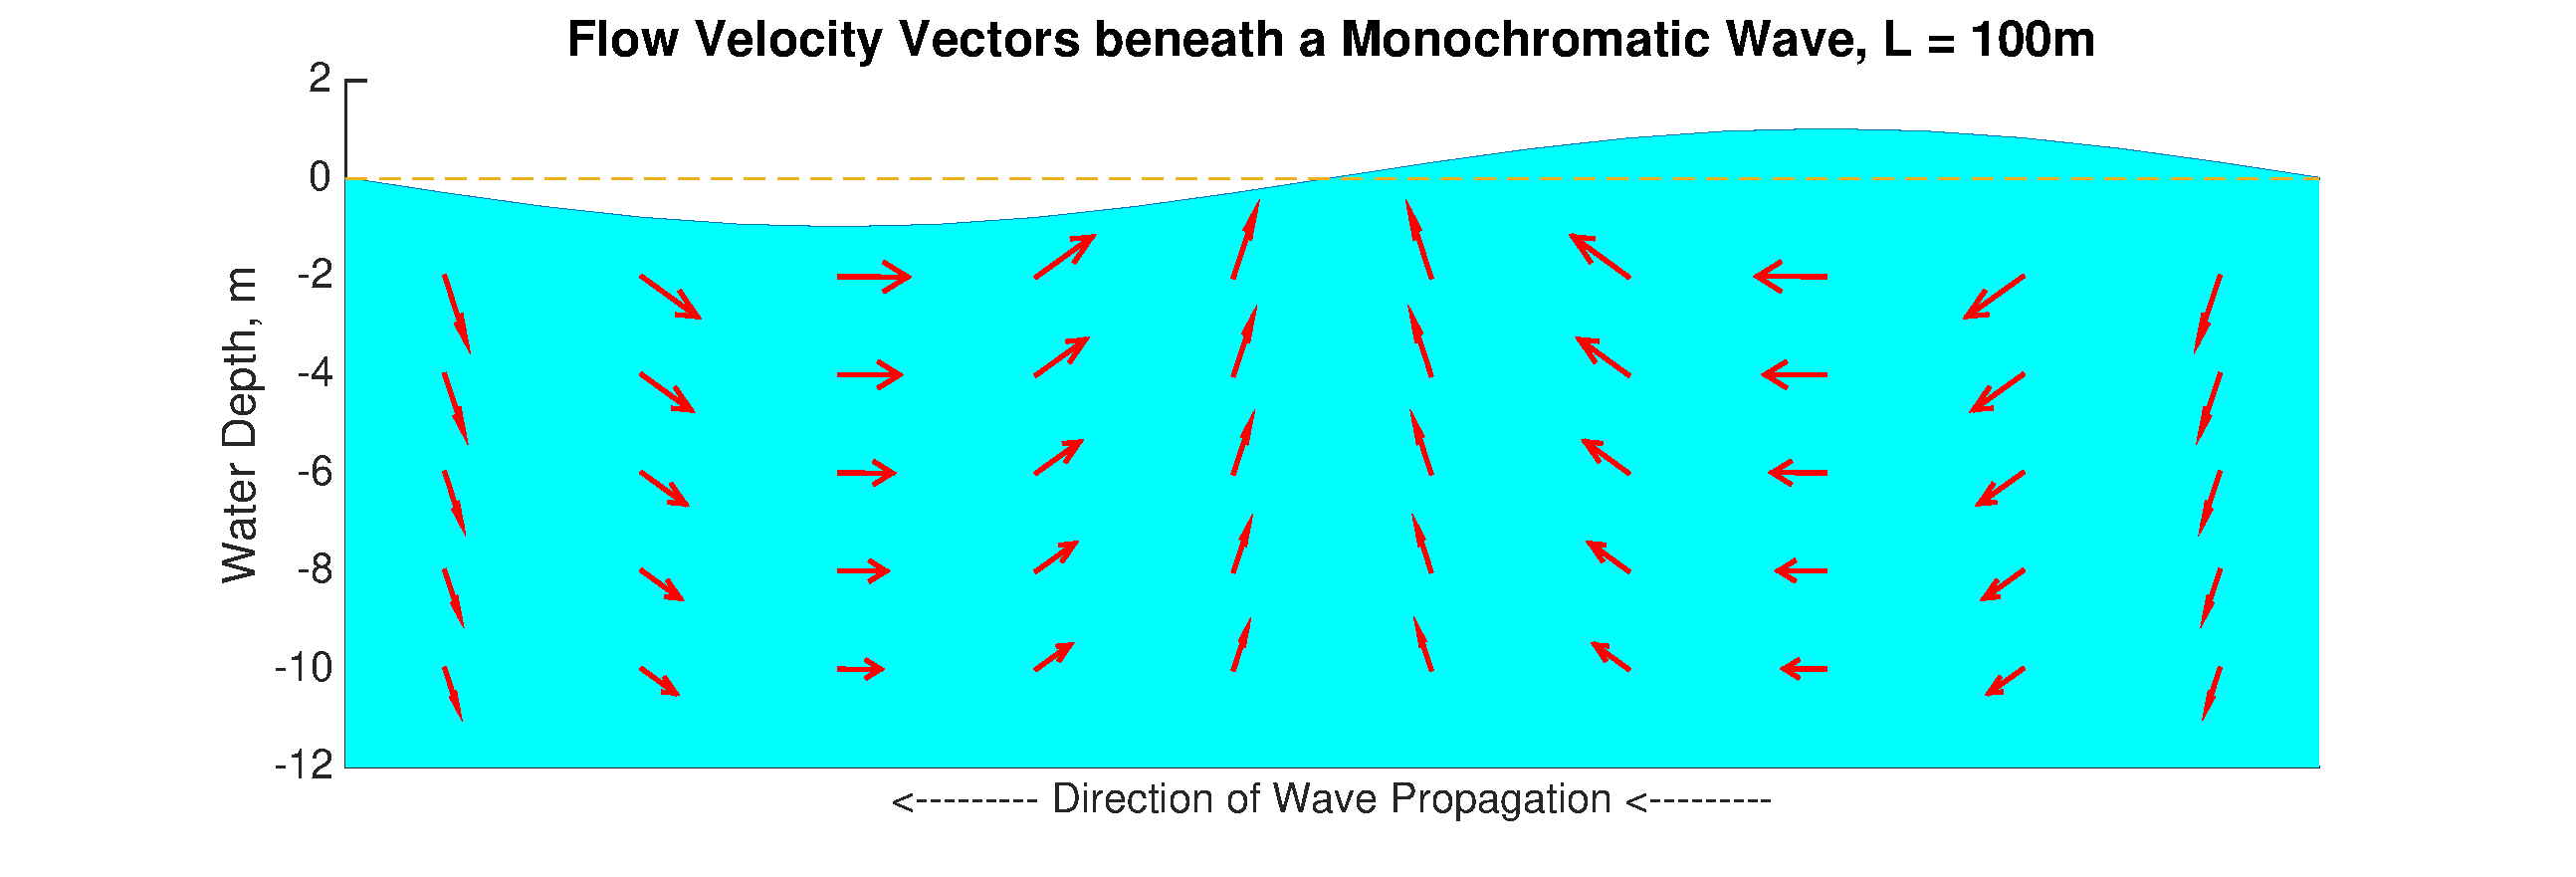
\includegraphics[width=1\columnwidth]{images/flowFig}
\vspace*{-16pt}
\centering
\caption{A visualization of the flow field velocity at various depths beneath a monochromatic wave. These vector lengths are not to scale and are intended to conceptualize the direction and decay with depth of wave forces.}
\centering
\label{fig:flowFig}
\end{figure}

The main novelty of the work presented in this paper is a control method that can forecast and compensate for future wave action. This is demonstrated through simulations of an underwater robot performing station keeping in a shallow water bathymetry under the influence of a strong sea swell. The calculated control actions are optimized to actuate an underwater robot's thrusters in an anticipatory fashion so that the vehicle remains nearly stationary as the waves pass over it. This allows us to increase the quality of robotic observations in shallow ocean water, as well as reducing the risk of equipment damage while deployed. MPC shows to reduce an underwater robot position error in a station keeping application when compared to traditional feedback control. Additionally, the algorithm is shown to be resistant to sensor noise of the observed wave field.

The remainder of this paper is organized as follows: related work is highlighted in Section~\ref{sec:related}. Next, the MPC method is described in Section~\ref{sec:mpc}. Section~\ref{sec:waves} describes the wave mechanics used in the system model. Section~\ref{sec:dynamics} outlines the vehicle model and overall system dynamics. Section~\ref{sec:sim} details the algorithm structure and controller specifics. Section~\ref{sec:results} presents results of determining effective prediction horizons and analyzes system performance against a simulated wave field with noisy observations. Finally, concluding remarks are provided in Section~\ref{sec:conclusion}. %Figure \ref{fig:structure} shows the paper outline in more detail. 

\section{Related Work}
\label{sec:related}

Path optimization is a pivotal aspect of robotic path planning where the amount of information gain should be maximized while considering some cost function, often times the mission duration. In \cite{smithtracking} and \cite{smithfront}, a sampling path is designed to minimize the distance between an AUV and specific oceanographic point of interests. The hybrid Fast Marching method, or FM*, employed in \cite{petres} uses an A* search heuristic to find a continuous path while minimizing water current drift. These methods incorporate water current models as a quadratic drag force, but do not include influence from wave forces. Localization challenges, such as the mid-column glider position uncertainty presented in \cite{medagodaADCP}, are further complicated when considering additive uncertainty due to wave disturbances.

Robotic maintenance of Wave Energy Converters (WEC), such as the platform detailed in \cite{joslin}, is an active area research. In fact, MPC techniques have been explored by the wave energy community as a way to optimize WEC power generation. As shown in \cite{brekken1} and \cite{brekken2}, MPC can incorporate actuator limits and system constraints to provide optimal energy capture while benefiting from a variable prediction horizon. Wave prediction modeling is also an active area of research. In \cite{ling}, Ling provides a method of real time WEC force estimation, showing accurate predictions for horizons up to \unit[15]{s}. This method is noteworthy since it does not require a network of sensors to provide wave information, as is often carried out. In \cite{colby}, Colby uses an artificial neural network to estimate wave forces from a hydrodynamic model as inputs to an evolutionary algorithm to optimize WEC geometry.

Applying MPC for underwater robotics is an enticing option as the combination of model dynamics and cost function minimization requires minimal tuning of controller gains. In \cite{huynh}, energy efficient paths for a glider are generated by minimizing costs across stratified, spatially-distributed currents using an A* search heuristic. In \cite{medagodaMPC}, MPC with a least squares cost function is used to optimize sawtooth paths for an underwater glider with an emphasis on real-time execution. This cost minimization technique is similar to that used in this paper. Both approaches show the value in state estimation for robotic path planning, but do not incorporate wave disturbances.

Wave-induced station keeping is explored in \cite{riedel1} and \cite{riedel2} where a dynamic Kalman filter is created to synthesize onboard sensor data to provide an estimate of wave-induced disturbances. This filter fuses ground speed from the Doppler Velocity Log (DVL), relative water speed from the Acoustic Doppler Current Profiler (ADCP), and attitude from the Inertial Measurement Unit (IMU) among other sensors to produce an estimate of the fluid velocity. This method highlights some of the difficulties of \textit{in situ} wave parameters. One drawback of their experiments was the need for a subsurface sensor network to provide wave parameters to the controller. The work in this paper seeks to improve on these results by providing improved cost minimization techniques and emphasizing real-time control execution.

\section{Model Predictive Control} 
\label{sec:mpc}

The term MPC does not refer to a specific strategy, but a variety of methods that all in some way incorporate the following \cite{camacho}:
\begin{itemize}
  \itemsep0.25em
  \item Modeled state estimator along some time horizon
  \item Cost function to minimize a control sequence 
  \item Receding horizon as optimized control is carried out 
\end{itemize}

MPC requires a model of the system dynamics that can estimate future states from a current state and set of control inputs along a time horizon. The model in this case includes the vehicle dynamics and thruster forces, along with a disturbance matrix to model the wave disturbances on the system. By thresholding the thruster forces within the minimization function, the need for tuning gains, such as in PID control, is removed \cite{rawlings}; however, the number of steps in the prediction horizon must be judiciously chosen. Too little time will not allow for the full dynamics of the system to be accounted for while too much time will be computationally intensive. 

The optimization objective is to find the sequence of input control actions to the state estimator that minimizes some global cost function. Cost functions can be formulated by balancing one or several metrics, e.g. mission duration, energy consumption, or number of sampled observations \cite{lavalle, binney}. Given the station-keeping objective, the cost function employed in this work is the sum of squared distances between the desired and predicted states added to its input control over the current horizon, or:
\begin{equation}
J = \sum_{k=1}^{N}[\vec{\Upsilon}_{target} - \vec{\Upsilon}_k(\vec{u}_k)]^2 + \vec{u}_k^2,
\label{eqn:cost}
\end{equation}
and
\begin{equation}
\vec{u}_{1:N}^* = \operatorname*{arg\,min}_{\vec{u}_{1:N}} J(\vec{u}_{1:N}),
\label{eqn:argmin}
\end{equation}
where $N$ is horizon length, $k$ is the current time step in the $N$ horizon, $\vec{\Upsilon}_{target}$ is the desired state, $\vec{\Upsilon}_k(u_k)$ is the state at time $k$ from input $\vec{u}_k$, and $\vec{u}_{1:N}^*$ is the optimized control input that minimizes the cost, $J$. 

The control action is then optimized by evaluating the Jacobian, which is the derivative of the cost with respect to the control action. The Jacobian is minimized as the optimal control action is approached. At each optimization step, a new set of control actions is generated by perturbing the previous set according to the Jacobian. The new control action effects are then estimated along the horizon. This is repeated until a set of control actions that minimizes the cost function is calculated as in \eqref{eqn:argmin}. This gradient descent method of cost evaluation and optimization is similar to that used by Medagoda et al. in \cite{medagodaMPC}.

\section{Wave Mechanics} 
\label{sec:waves}

According to Linear Wave Theory (LWT), a wave field in a random sea is composed of a superposition of sinusoids. Once decomposed, each sinusoid can then be analyzed as a single monochromatic wave with unique period ($T$), amplitude ($a$), and phase offset ($\phi$) \cite{phillips,D&D}. For reference, this paper instead uses the term waveheight ($H$), which is simply twice the amplitude ($H = 2a$). LWT assumes fluid flow is irrotational, incompressible, and inviscid, thus allowing for potential flow \cite{bosma}. In practice, LWT is not only easily implemented, but has also been shown to produce surprisingly accurate results \cite{D&D}. Thus, LWT is often employed for a reliable primary analysis before other nonlinear theories, and it forms the wave action model used in this paper.

Using LWT, a field of random sea waves, not unlike an electrical signal, can be decomposed to its component frequency spectra by way of a Discrete Fourier Transformation (DFT) \cite{goda}. DFT solvers will output frequency parameters with associated energies correlating to signal amplitude. The phase information can then be extracted by taking the $tan^{-1}$ of the imaginary over the real part of each component. For details on Fourier spectra of wave fields, see \cite{falnes}. 

In this work, the input wave field is assumed to be provided to the vehicle as an array of wave period, wave height, and phase offset ($T, H, \phi$). Component wavelengths ($L$), wave numbers ($k$), and frequencies ($\omega$) are solved for by way of the dispersion relation \cite{D&D}. The superimposed wave field shown in Fig.~\ref{fig:eta} is then constructed by the water surface wave equation shown below: 
 
\begin{equation} 
\eta(\vec{t}) = \sum \frac{H}{2}cos(k\vec{x}-\omega\vec{t}+\phi) .
\label{eqn:eta}
\end{equation}

Beneath each component monochromatic wave, wave-induced particle displacements occur in a cyclical fashion. In deep water waves where depth is greater than approximately half of the wavelength ($d > L/2$), these displacements follow circular paths. As $d$ decreases, the paths become more elliptical until they are nearly horizontal in the surf zone \cite{D&D}. Associated particle velocities and accelerations can be derived from these trajectories. As stated earlier, the magnitude of these velocities and accelerations decay exponentially through the water column such that they are negligible ($< 0.04\%$) at a depth, $d \approx L/2$ \cite{D&D}. The per-wave, at-depth solutions to these velocity and acceleration equations are used as the primary inputs to the modeled system dynamics.

\section{System Dynamics} 
\label{sec:dynamics}

For the scope of this paper, the term Remotely Operated Vehicle (ROV) will be used to describe a tethered unmanned vehicle whose operation may or may not be tele-operated \cite{ROV}. The ROV modeled for this work is the SeaBotix vLBV300 shown in Fig.~\ref{fig:seabotix}. In simulation, the ROV is not tele-operated and performs control actions autonomously.

\begin{figure}
\includegraphics[width=0.8\columnwidth]{images/volt}
\centering
\caption{A SeaBotix vLBV300 ROV similar to the one modeled in this work. Along with IMU and DVL sensors, the vehicle has six angled thrusters which control it along five degrees of freedom: heave (vertical $z$), sway (lateral $y$), surge (lateral $x$), roll (rotation around $x$), and yaw (rotation around $z$).}
\centering
\label{fig:seabotix}
\end{figure}

\begin{table}
\caption{Vehicle parameters used in simulation}
\begin{center}
\def\arraystretch{1.2}%
\begin{tabular}{ |l|c|c| } 
 \hline 
 Parameter & Symbol & Value \\ 
 \hline
 Density of Seawater & $\rho_{sea}$ & $1030~kg/m^3$ \\ 
 Incident Area, $\vec{x}$ & $A_{i,\vec{x}}$ & $0.156~m^2$ \\ 
 Incident Area, $\vec{z}$ & $A_{i,\vec{z}}$ & $0.273~m^2$ \\
 Moment of Inertia, $\vec{x}$ & $I_{xx}$ & $0.62~kg~m^2$ \\
 Moment of Inertia, $\vec{z}$ & $I_{zz}$ & $1.60~kg~m^2$ \\
 Dry Mass & $m_{dry}$ & $22.2~kg$ \\
 Added Mass, $\vec{x}$ & $m_{add,x}$ & $8.1~kg$ \\
 Added Mass, $\vec{z}$ & $m_{add,z}$ & $36.7~kg$ \\
 Drag Coefficient, $\vec{x}$ & $c_{d,x}$ & $0.84$\\
 Drag Coefficient, $\vec{z}$ & $c_{d,z}$ & $1.06$\\
 Max Thruster Force & $T_{max}$ & $29.7~N$ \\
 Thruster Angle, Forward & $\theta_f$ & $35\degree$ \\
 Thruster Angle, Aft & $\theta_a$ & $45\degree$ \\
 Thruster Angle, Vertical & $\theta_v$ & $20\degree$ \\
 \hline
\end{tabular}
\end{center}
\label{table:vehicleData}
\end{table}

\subsection{Vehicle Model}

The SeaBotix vLBV300 ROV has six vectored thrusters controlling motion along five degrees of freedom. For the scope of this work, only the surge and heave directions, or forward (global $\vec{x}$) and vertical (global $\vec{z}$) axes, are considered. See Fig.~\ref{fig:seabotix} for reference. 

The vehicle is assumed to be a rigid body, and irrotational in the water flow. Since its size is well below the wavelength, its drift motion is assumed to follow that of a particle. Vehicle dimensions, mass parameters, and thruster forces are provided in Table~\ref{table:vehicleData}. Moment of inertia and center of gravity data was provided by a CAD model input to Dassault Systèmes SolidWorks \cite{solidworks}. Added mass values were provided by the same model input to Ansys AQWA \cite{aqwa}. Drag coefficient data was provided by the manufacturer. The differential equation defining ROV motion is: 
\begin{equation}
\vec{M}\dot{\vec{v}}_a + \vec{F}_d + \vec{F}_g + \vec{F}_c = \vec{F}_{thrust},
\label{eqn:forceBal1}
\end{equation}
where $\vec{M}$ is a mass term containing the dry and added masses, $m_{dry}$ and $m_{add}$, $\vec{v}_a$ is the absolute velocity of the vehicle with respect to the inertial reference frame, $\vec{F}_d$ is the drag force from the water, $\vec{F}_g$ is the force of gravity, $\vec{F}_c$ is the Coriolis force, and $\vec{F}_{thrust}$ is the ROV thruster force. By assuming that the Coriolis force is negligible and that the vehicle is neutrally buoyant, the $\vec{F}_c$ and $\vec{F}_g$ terms are neglected. Substituting inertia and drag relations, \eqref{eqn:forceBal1} becomes: 
\begin{equation}
m_{dry} \dot{\vec{v}}_a + m_{add} \dot{\vec{v}}_r - \frac{1}{2} \rho_{sea} A_i c_d \abs{\dot{\vec{v}}_r} \dot{\vec{v}}_r = \vec{F}_{thrust},
\label{eqn:forceBal2}
\end{equation}
where $\vec{v}_r$ is the velocity of the vehicle relative to the water, which acts on the added mass term of $\vec{M}$ in \eqref{eqn:forceBal1}. Substituting heave, surge, and particle velocity components, \eqref{eqn:forceBal2} becomes:
\begin{equation}
\begin{split}
\vec{F}_{thrust} = \begin{bmatrix} m_{dry}+m_{add,\vec{x}} \\ m_{dry}+m_{add,\vec{z}} \end{bmatrix} \begin{bmatrix} \ddot{\vec{x}} \\ \ddot{\vec{z}} \end{bmatrix} - \begin{bmatrix} m_{add,\vec{x}} \\ m_{add,\vec{z}} \end{bmatrix} \begin{bmatrix} \dot{\vec{v}}_{p,\vec{x}} \\ \dot{\vec{v}}_{p,\vec{z}} \end{bmatrix} \\- \frac{\rho_{sea}}{2} \begin{bmatrix} A_{i,\vec{x}}C_{d,\vec{x}} \\ A_{i,\vec{z}}C_{d,\vec{z}} \end{bmatrix} \begin{bmatrix} \abs{\dot{\vec{x}}-\vec{v}_{p,\vec{x}}} (\dot{\vec{x}}-\vec{v}_{p,\vec{x}}) \\ \abs{\dot{\vec{z}}-\vec{v}_{p,\vec{z}}} (\dot{\vec{z}}-\vec{v}_{p,\vec{z}}) \end{bmatrix},
\label{eqn:forceBal3}
\end{split}
\end{equation}
where $\vec{v}_p$ is the particle velocity at a time and position beneath a monochromatic wave. For added reference, $\vec{v}_a$ = $\vec{v}_r$ + $\vec{v}_p$, and $\dot{\vec{v}}_{a,\vec{x}}$ = $\ddot{\vec{x}}$, $\dot{\vec{v}}_{a,\vec{z}}$ = $\ddot{\vec{z}}$.

\subsection{State Space Form}

The differential equations are now rewritten in state space form solvable by the simulator. This takes the form:
\begin{equation}
\dot{\vec{\Upsilon}} = \begin{bmatrix} \dot{\vec{x}} & \ddot{\vec{x}} & \dot{\vec{z}} & \ddot{\vec{z}}\end{bmatrix}^T = \vec{A}\vec{x} + \vec{B}\vec{u} + \vec{D},
\label{eqn:SS_all}
\end{equation}
where
\begin{equation}
\vec{A}\vec{x} = \begin{bmatrix} 0 & 1 & 0 & 0 \\ 0 & 0 & 0 & 0 \\ 0 & 0 & 0 & 1 \\ 0 & 0 & 0 & 0  \end{bmatrix} \begin{bmatrix} \vec{x} \\ \dot{\vec{x}} \\ \vec{z} \\ \dot{\vec{z}} \end{bmatrix},
\label{eqn:SS_A}
\end{equation}
\begin{equation} 
\vec{B}\vec{u} = \scalemath{0.67}{ \frac{T_{max}}{m_{dry}} \begin{bmatrix} 0 & 0 & 0 & 0 & 0 & 0 \\ cos\theta_f & cos\theta_f & -cos\theta_a & -cos\theta_a & 0 & 0 \\ 0 & 0 & 0 & 0 & 0 & 0 \\ 0 & 0 & 0 & 0 & -cos\theta_v & -cos\theta_v \end{bmatrix} \begin{bmatrix} u_1 \\ u_2 \\ u_3 \\ u_4 \\ u_5 \\ u_6 \end{bmatrix} },
\label{eqn:SS_B}
\end{equation}
and
\begin{equation} 
\vec{D} = \scalemath{0.99}{\begin{bmatrix} 0 \\ \frac{\dot{\vec{v}}_{p,\vec{x}}}{m_{dry}} + \frac{\rho_{sea} A_{i,\vec{x}} C_{d,\vec{x}}}{2(m_{dry}+m_{add,\vec{x}})} \abs{\dot{\vec{x}}-\vec{v}_{p,\vec{x}}} (\dot{\vec{x}}-\vec{v}_{p,\vec{x}})  \\ 0 \\ \frac{\dot{\vec{v}}_{p,\vec{z}}}{m_{dry}} + \frac{\rho_{sea} A_{i,\vec{x}} C_{d,\vec{z}}}{2(m_{dry}+m_{add,\vec{z}})} \abs{\dot{\vec{z}}-\vec{v}_{p,\vec{z}}} (\dot{\vec{z}}-\vec{v}_{p,\vec{z}}) \end{bmatrix}}. 
\label{eqn:SS_D}
\end{equation}

The $\vec{u}$ vector in \eqref{eqn:SS_B} refers to motor inputs of each of the vehicle's six vectored thrusters: $u_1$ and $u_2$ are the forward thrusters, $u_3$ and $u_4$ are the aft thrusters, and $u_5$ and $u_6$ are the vertical thrusters.

\section{Simulator Setup}
\label{sec:sim}

The ROV was simulated along a \unit[240]{s} long time vector with \unit[0.2]{s} discretizations. All robot thruster actuations and wave disturbances occur along the global $\vec{x}$ and $\vec{z}$ axes. Each motor input simulated by the $\vec{B}\vec{u}$ matrix in \eqref{eqn:SS_B} is a thresholded value between [-1,1], which correlates to a percentage of maximum possible thrust. All forward-looking state estimations and robot movements use the MATLAB function \Call{ode45}{} which uses a variable step Runge-Kutta Method to numerically solve the system differential equations \cite{ode45}.

\subsection{Wave Field Model} 

The bathymetry and wave climate selected for analysis is similar to that of the National Northwest Marine Renewable Energy Center (NNMREC) North Energy Test Site (NETS) in the coastal Pacific Ocean two nautical miles out of Newport, Oregon \cite{ling}. The operational depth at NETS is approximately \unit[50]{m}. The wave field used in this work was qualitatively verified using AWAC acoustic measurement data deployed at NETS in August 2013. Each \unit[40]{min} time series was recorded at \unit[2]{Hz}.

The wave field used by the simulator is the set of eight different periods, heights, and phases ($T, H, \phi$) detailed in Table~\ref{table:waveData}. By assuming LWT and using superposition, a reconstructed time series using \eqref{eqn:eta} is shown in Fig.~\ref{fig:eta}. Because of the 2-dimensional analysis along only surge and heave motions, wave angles are set to 0.

\setlength\tabcolsep{5pt}
\begin{table}
\caption{Wave field parameters used in simulation}
\begin{center}
\def\arraystretch{1.1}%
\begin{tabular}{ |l|c|c|c|c|c|c|c|c|c| } 
 \hline 
 Component Wave & 1 & 2 & 3 & 4 & 5 & 6 & 7 & 8 \\ 
 \hline
 Wave Period, s & 10 & 8 & 12 & 11 & 6 & 7 & 9 & 25  \\ 
 Wave Height, m & 1.8 & 0.9 & 1.6 & 1.3 & 0.4 & 0.5 & 1.1 & 0.7 \\ 
 Phase, radians & -$\frac{\pi}{2}$ & -$\frac{\pi}{4}$ & -$\frac{5\pi}{8}$ & $\frac{4\pi}{13}$ & -$\frac{\pi}{15}$ & $\frac{\pi}{3}$ & -$\frac{\pi}{18}$ & -$\frac{7\pi}{4}$\\
 \hline
\end{tabular}
\end{center}
\label{table:waveData}
\end{table}

\begin{figure}
\includegraphics[width=1\columnwidth]{images/eta}
\vspace*{-14pt}
\centering
\caption{A time series of the wave profile over the 240~s simulated time window constructed using the parameters listed in Table \ref{table:waveData}.}
\label{fig:eta}
\end{figure}

Prior to any forward state estimation or any simulated vehicle motion, the wave action, or particle accelerations and velocities, are calculated for the robot's current position in time and space. These accelerations and velocities are calculated for each wave and summed by superposition in the function \Call{getParticles}{} shown in Algorithm~\ref{alg:MPC}.

\subsection{Algorithm Layout}

The \Call{MPC}{} algorithm shown in Algorithm~\ref{alg:MPC} requires four inputs. The first, $t$, is a time object containing the overall time vector and horizon and discretization parameters. The second input, $\lambda$, is an object containing all relevant wave spectra data. The third input is the robot object, which contains the vehicle dynamics, states, and error history. The last input, $\Upsilon_{target}$, is the target state.

\begin{algorithm}
\caption[caption]{MPC for ocean wave station keeping \hspace{\textwidth}where $t$ is a time vector, $\lambda$ is an object containing all relevant wave spectra data, and $\Upsilon$ represents states in time and space.}
\label{alg:MPC}
\begin{algorithmic}[1]

\Procedure{$MPC$}{ $t$, $\lambda$, robot, $\Upsilon_{target}$ } 
\State $n\gets1$
\State $\eta \gets$ \Call{loadSeaState}{ $t$, $\lambda$, $\Upsilon_{initial}$ }
\While{$n<$ simulatorOff}
\State input $\gets$ \Call{getForecast}{$t$, robot, $\lambda$, $\Upsilon_{target}$, $n$} 
\State robot $\gets$ \Call{moveRobot}{ $t$, robot, $\lambda$, input, $n$ } 
\State $n \gets n+1$
\EndWhile
\EndProcedure

\Function{getForecast}{ $t,$ robot, $\lambda, \Upsilon_{target}, count$ }
\State $i \gets 1$
\State $N \gets t.Horizon$ / $t.Discretization$
\State $J_i$, $u_i$, $\Upsilon_i \gets$ \Call{initializeInput}{ robot }
\State $\delta \gets$ \Call{initializeDelta}{ } 
\While{$i$ < maxIterations \textbf{and} $\delta$ > exitCriteria}
\State $u_{i+1} \gets u_{i} - \delta$
\For {$k\in [1,2,...,N]$}
\State $\vec{v}_p, \dot{\vec{v}}_p \gets$ \Call{getParticles}{ $t$, $\Upsilon_i(k)$, $\lambda$ }
\State $\Lambda \gets \vec{v}_p, \dot{\vec{v}}_p$
\State $\Upsilon_{i+1}(k) \gets$ \Call{getState}{$t$, robot, $\Lambda$, $u_{n+1}(k)$}
\State $J_{i+1}(k) \gets$ \Call{getCost}{ $\Upsilon_{target}$, $\Upsilon_{i+1}(k)$ }
\EndFor
\State $\delta \gets$ \Call{getJacobian}{ $J_i$, $J_{i+1}$, $u_i$, $u_{i+1}$ }
\State $u_i \gets u_{i+1}$
\State $J_i \gets J_{i+1}$
\State $\Upsilon_i \gets \Upsilon_{i+1}$
\State $i \gets i+1$
\EndWhile
\State \Return $u_{i+1}$
\EndFunction

\end{algorithmic}
\end{algorithm}

Once all inputs are passed through, \Call{MPC}{} runs by first generating the initial sea state at \Call{loadSeaState}{} from the wave spectra data in $\lambda$. Then, and until some cessation criteria, \Call{getForecast}{} generates the optimized motor inputs for each thruster while \Call{moveRobot}{} passes those inputs and moves the robot one step forward along that control vector. 

In \Call{getForecast}{}, the function \Call{initializeInput}{} generates initial cost, control, and state vectors, or $J_i$, $\vec{u}_i$, and $\vec{\Upsilon}_i$ respectively. The initial control vector, $\vec{u}_i$, is a set of PD control actions along the $N$ horizon. \Call{initializeDelta}{} creates a value, $\delta$, to perturb $\vec{u}_i$ and generates a new input, $\vec{u}_{i+1}$, which is then evaluated. First, the wave forces along the input trajectory, $\vec{v}_p$ and $\dot{\vec{v}}_p$, are calculated through \Call{getParticles}{}. Next, $\vec{v}_p$, $\dot{\vec{v}}_p$, and the control vector, $\vec{u}_{i+1}$ are passed in to \Call{getState}{} which estimates the resulting predicted state, $\vec{\Upsilon}_{i+1}$. Lastly, $\vec{\Upsilon}_{i+1}$ is evaluated with respect to the target state, $\vec{\Upsilon}_{target}$ in \Call{getCost}{} by way of the cost function in \eqref{eqn:cost}.

After the cost, $J_{i+1}$, is evaluated over the entire $N$ horizon, the function \Call{getJacobian}{} evaluates the Jacobian, or $\partial \vec{J} / \partial \vec{u}$, and returns a new $\delta$ value. This value translates the rate at which cost changes with respect to a change in control inputs, and a $\delta$ value growing smaller implies that a control vector is nearing a local minimum. At the end of each evaluation, if $\delta$ does not meet some $exitCriteria$, a new input vector is generated and the process is repeated. If it does; however, the optimized control vector, $\vec{u}_{i+1}$, is returned and the robot moves forward along that trajectory. 

\section{Results} 
\label{sec:results}

One challenge when implementing MPC is determining a preferred prediction horizon. Section~\ref{results:bestHorizon} details how the horizon that balances solution accuracy with computation time is selected for this work. Section~\ref{results:perform} evaluates the controller with the chosen prediction horizon against a standard PD controller in the same wave climate. Finally, in Section~\ref{results:noise}, sensor observation noise is inserted to the MPC and is compared with the deterministic PD controller. For all simulations, the robot was to maintain a depth of $\vec{z} = \unit[-15]{m}$ below the surface, or $\Upsilon_{target} = [0, -15]$. The simulator is designed to simulate wave forces at any depth; however, simulations were not run at varied depths as the scaled results offered little additional insight. The $exitCriteria$ for an optimized trajectory used in Algorithm~\ref{alg:MPC} was set to \unit[5]{mm}. 

\subsection{Determination of Prediction Horizon} \label{results:bestHorizon}

A good prediction horizon for MPC should reasonably balance computation time against position error. This is a discretionary characteristic as certain implementations may have stricter tolerances than others. In this work, simulations were run with a horizon ranging from \unit[0.2]{s} to \unit[3.0]{s}. Table~\ref{table:bestHorizon} shows total RMS errors and computation times per horizon. 

\setlength\tabcolsep{4pt}
\begin{table}[h]
\caption{Performance of various simulated horizons}
\begin{center}
\def\arraystretch{1.2}%
\begin{tabular}{ |l|c|c|c|c|c|c|c| } 
 \hline 
 Horizon, s & 0.2 & 0.4 & \textbf{0.8} & 1.0 & 1.6 & 2.0 & 3.0 \\ 
 \hline
 $Error_{RMS}$, m & 2.26 & 0.94 & \textbf{0.35} & 0.29 & 0.13 & 0.02 & 4.0$E$-6 \\ 
 $\Sigma$ $time_{Calc}$, s & 1658 & 507.1 & \textbf{93.8} & 233.2 & 7808 & 21886 & 101252 \\ 
 \hline
\end{tabular}
\end{center}
\label{table:bestHorizon}
\end{table}
\setlength\tabcolsep{6pt}

Based on the information in Table~\ref{table:bestHorizon}, two potential choices for prediction horizon are 0.8 and \unit[1.0]{s}. Both of these offer low RMS error at reasonable computation times. For the results presented in this work, the chosen horizon time was \unit[0.8]{s} as it yielded only a \unit[6]{cm}m difference in error for less than half the total computation time. 

With regards to the \unit[1.0]{s} horizon, it is worth noting that the \unit[240]{s} long time vector used in simulation is just longer than the \unit[233.2]{s} run time needed. This presents challenges when considering real-time implementation of this method. One solution is to recalculate the next optimized trajectory not at each \unit[0.2]{s} time step, but one or multiple steps later. In practice, the robot would use the first two or three inputs from the optimized control vector instead of just the first, while simultaneously calculating the next trajectory. This would lead to fewer calculations but may increase overall error due to sensor drift. 

Another result worth noting is the long run times from the shorter horizon controllers (0.2 and \unit[0.4]{s}). They showed poor performance, resulting in significantly larger tracking error and requiring several times more calculation time than the chosen horizon of \unit[0.8]{s}. This is likely due to an induced "myopia" where: 1) the robot does not properly account for its own inertia and 2) the robot does not take proper advantage of changes in flow direction. 

As expected, the longer horizons yield reduced errors at the expense of computation time. None of the later three time horizons (1.6, 2.0, and \unit[3.0]{s}) were considered because of unreasonable time costs. An obvious avenue for future work is to implement faster optimization and programming techniques to further increase the robot horizon.

\begin{figure*}
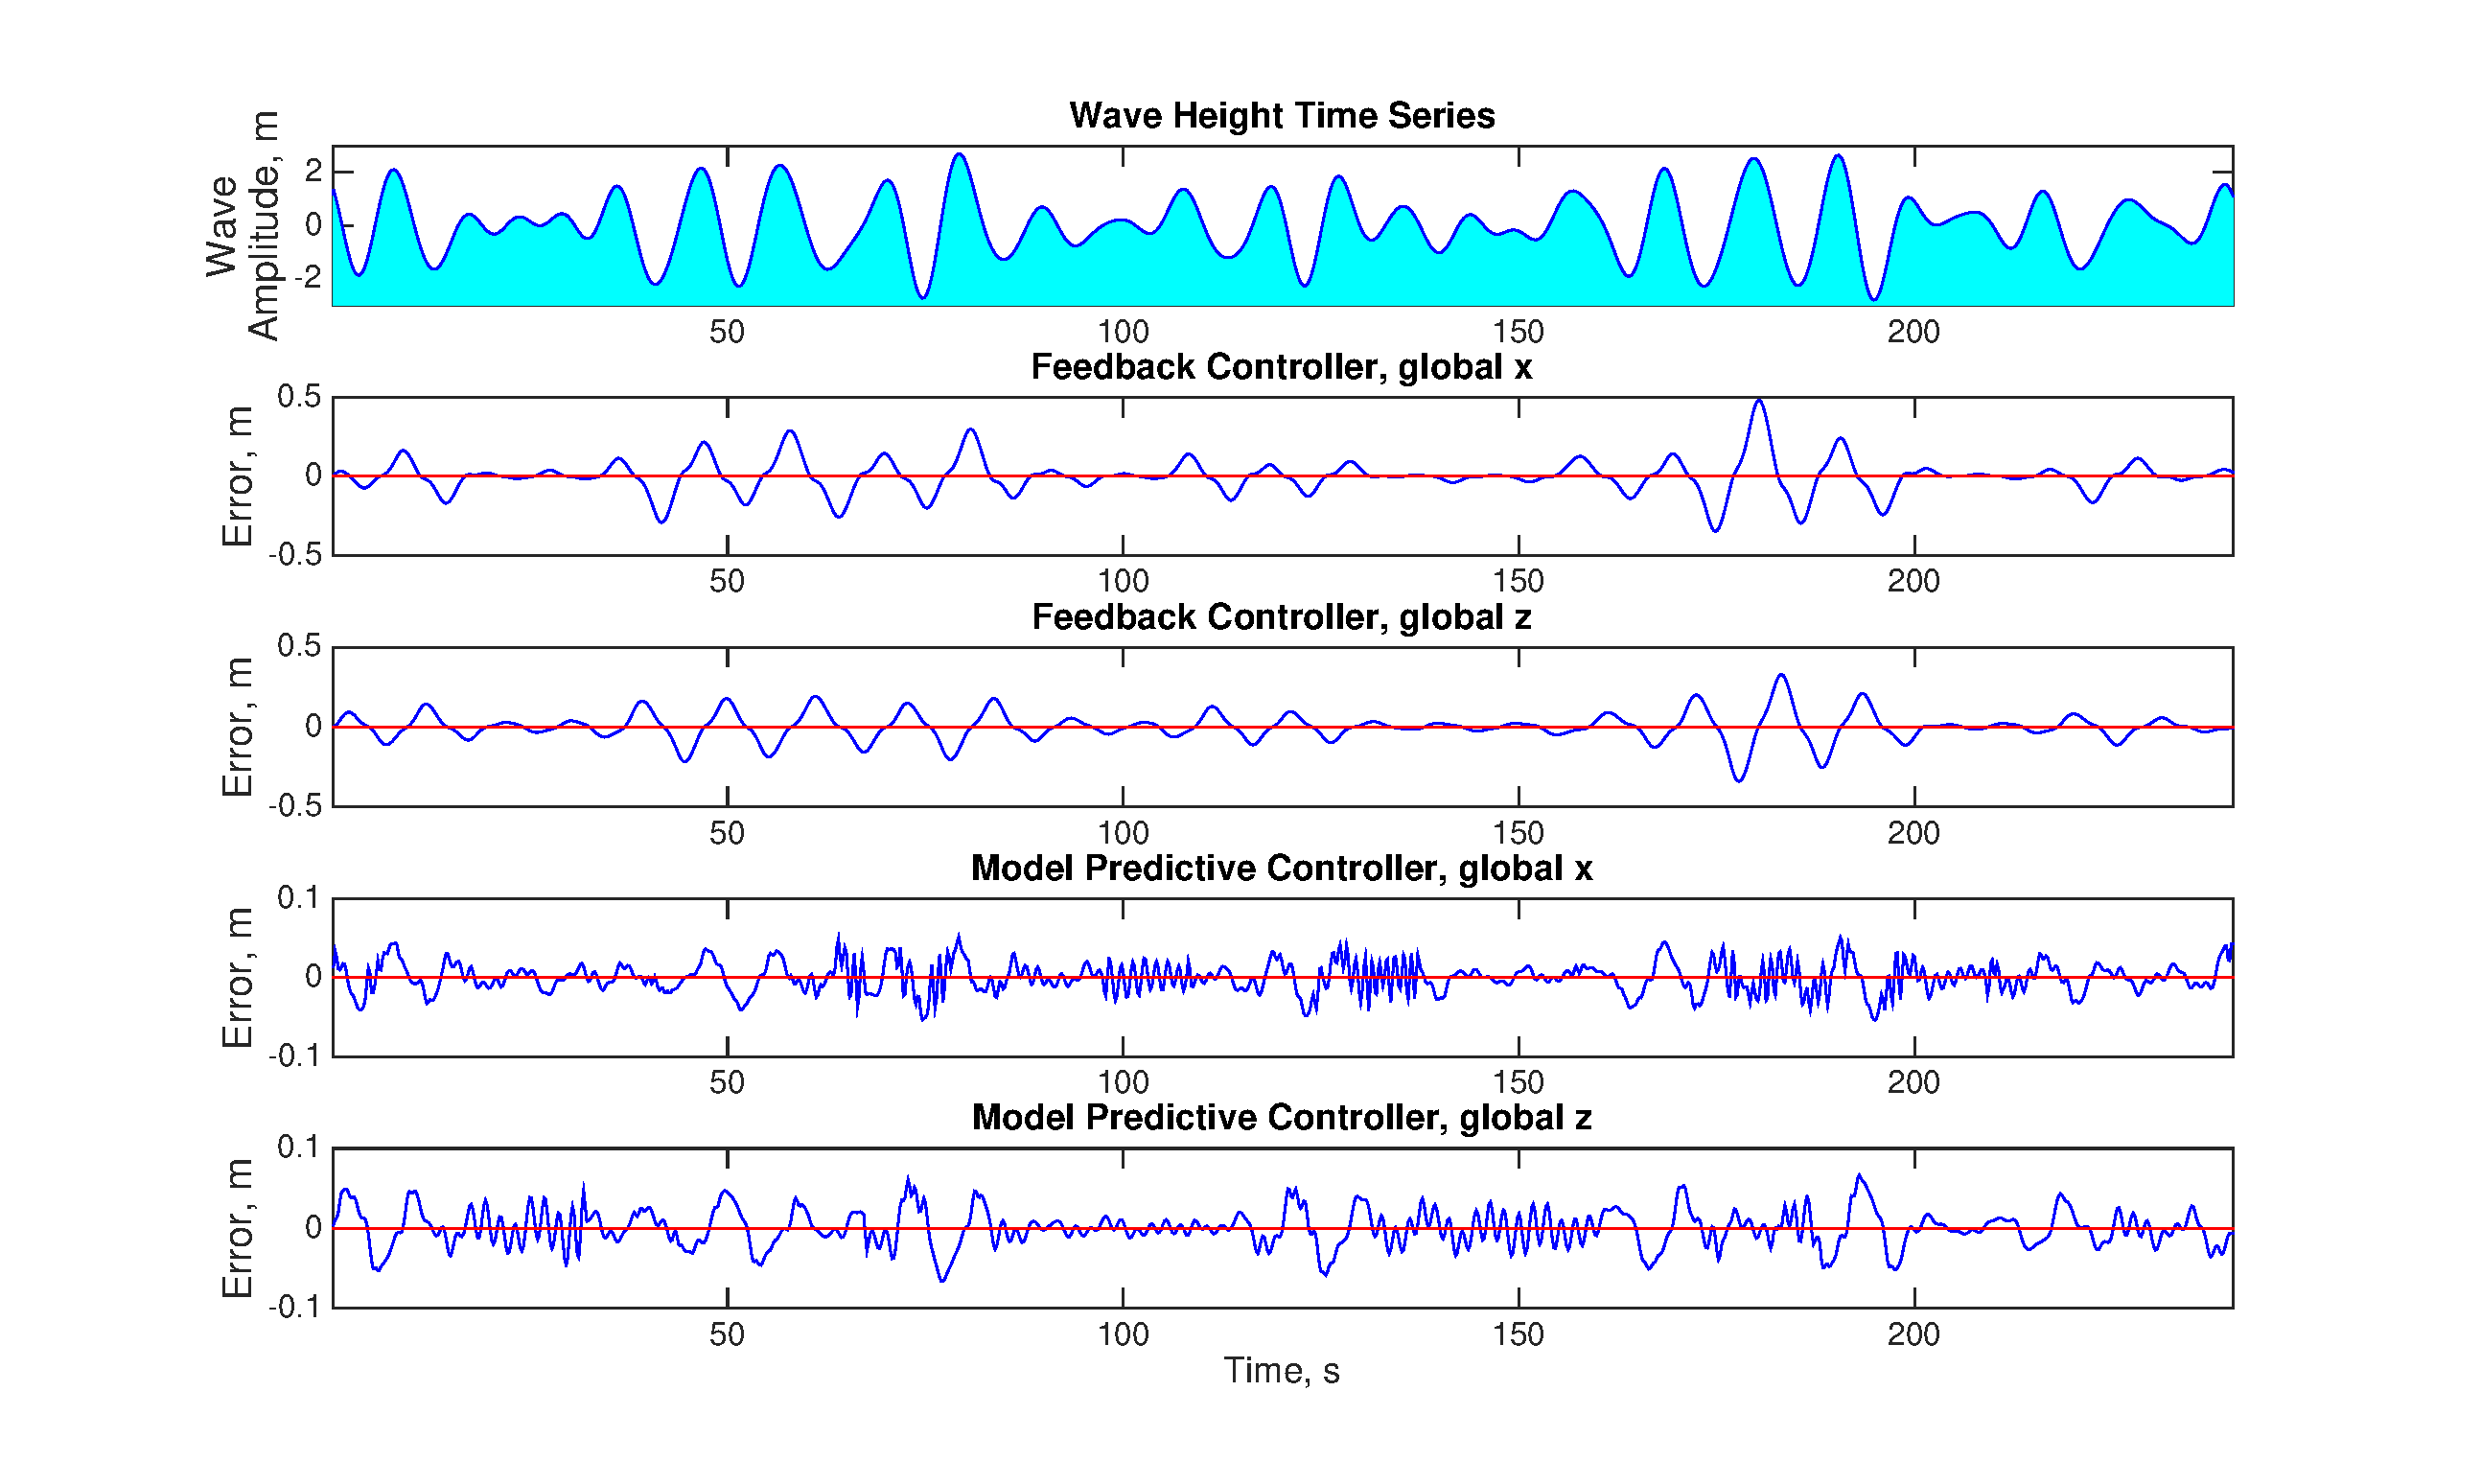
\includegraphics[width=1\linewidth]{images/compFig}
%\vspace*{-14pt}
\centering
\caption{Position error time series in global $\vec{x}$ and $\vec{z}$ coordinates when comparing a traditional feedback controller with a model predictive controller. As shown, MPC returns error values \unit[74]{\%s} lower than PD Control. RMS error values for these results are shown in Fig~\ref{fig:errorsBar}.} 
\label{fig:errorComp}
\end{figure*}

\subsection{MPC Performance} \label{results:perform}

Another set of simulations was run where a robot employing an \unit[0.8]{s} horizon MPC was compared against one using a traditional PD controller. Both were tested under the influence of the same wave field. Additionally, a free-floating, non-actuated robot disturbed by the same waves was simulated and compared for reference. Figure~\ref{fig:errorComp} details the positional errors for the PD and MPC controllers over the length of simulated time and Fig.~\ref{fig:errorsBar} shows the RMS error for each case.

As shown in Fig.~\ref{fig:errorComp}, MPC gives a \unit[74]{\%} reduction in position error over PD control. This substantial reduction is attained because the robot state estimator minimizes cost by using thrusters in an anticipatory action. In practice, the robot would thrust "against" the wave to reduce net displacement. Without any forward-looking state estimation, the PD controller can only choose a direct trajectory towards the desired state that is always deviated by the wave action.  

In Fig.~\ref{fig:errorComp}, the wave field time series is provided to show the correlation between wave height, $H$, which is directly proportional with wave forces in the water column \cite{D&D}, and position error below the waves. Both the MPC and PD controllers record little error as $H$ approaches zero, which is expected. As $H$ increases; however, the PD errors increase at a larger rate than the increase in MPC errors. This again results from the state estimator's ability to predict changes in flow direction and the impending effects of those changes on the robot's inertia.

\begin{figure}
\includegraphics[width=1\columnwidth]{images/errorsBar}
\vspace*{-16pt}
\centering
\caption{RMS errors for the three cases in Section \ref{results:perform}. The MPC robot showed a \unit[74]{\%} reduction in error compared to another using PD control.}
\label{fig:errorsBar}
\end{figure}

\begin{figure}
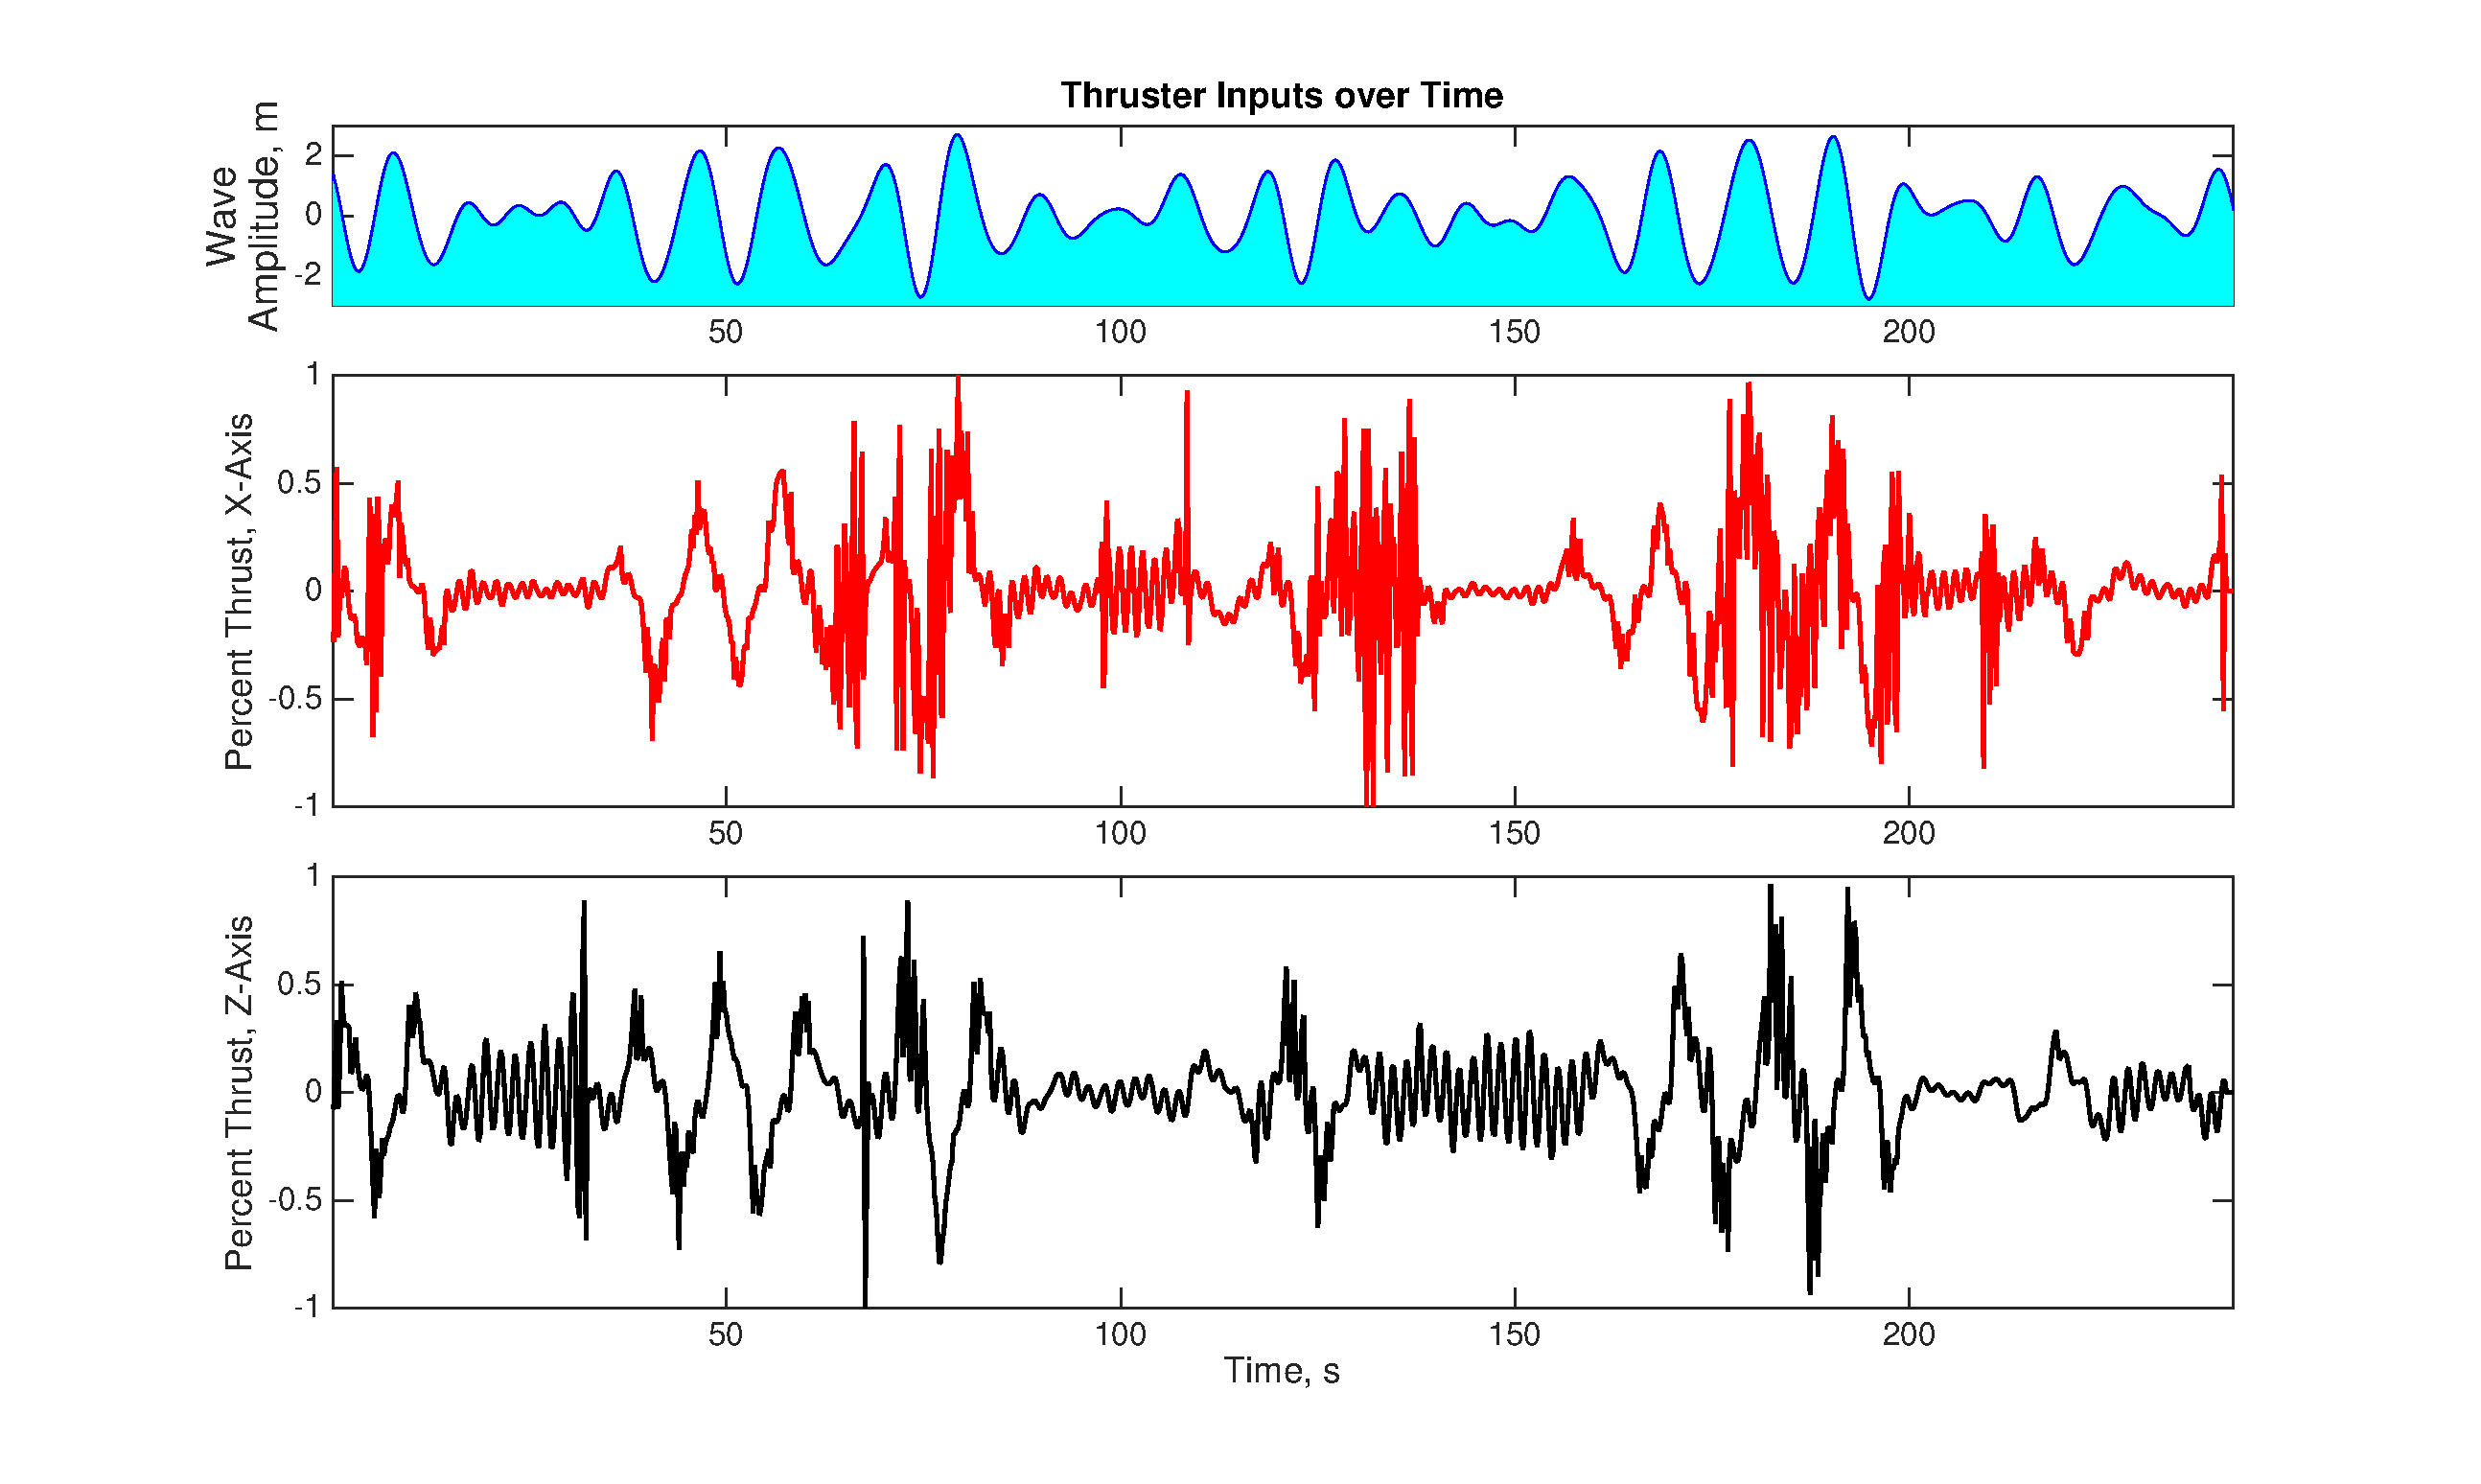
\includegraphics[width=1\columnwidth]{images/thrusts}
%\vspace*{-14pt}
\centering
\caption{MPC thruster inputs in global $\vec{x}$ and $\vec{z}$ coordinates over the simulated time series. The controller does not issue commands that saturate the thrusters for prolonged periods; however, it is prone to frequent direction changes.}
\label{fig:thrusts}
\end{figure}

Figure~\ref{fig:thrusts} shows a time series of thruster inputs in percentages of maximum thrust. As expected, the controller issues less thrust when the wave action is reduced. This is a result of the added input term to the cost function minimized in \eqref{eqn:cost}. One concern about the inputs shown is that there are frequent changes in direction. This can lead to unrealistic results as thruster actuation time was not considered in this work. A better model of thruster dynamics as well as an updated cost function to penalize large changes in thruster input are both avenues for future work.

\subsection{Sensor Noise Impact} \label{results:noise}

Simulations were also carried out to compare optimized trajectories to the effects of simulated sensor observation noise. For this set, Gaussian noise is injected to the vehicle's perceived value of particle velocities and accelerations, $\vec{v}_p$ and $\dot{\vec{v}}_p$. The wave field parameters were selected instead of other forms of localization noise because the vehicle Inertial Measurement Unit (IMU) has lower resolution than the Doppler Velocity Log (DVL), thus it is more likely that the IMU would give inaccurate observations on the pressure field above it (the wave action) than the DVL with bottom lock would on vehicle localization. By extension, this assumption allows for the PD control data from Section~\ref{results:perform} to serve as a deterministic basis of comparison.

The additive, independent, and identically-distributed Gaussian noise is provided by the MATLAB function \Call{awgn}{}. This function injects noise to the desired signal according to a Signal-to-Noise Ratio (SNR) which is related to the noise variance. For this simulation, the wave height, $H$, was assigned the highest variance to account for the moderately noisy heave data provided by the deployed buoy sensors \cite{goda}. Noise with a smaller variance is injected into the wave period, $T$, and phase terms, $\phi$, to account for error in Fourier coefficients and their resulting phase transformations.

\begin{table}[h]
\caption{Performance of MPC with noisy wave observations}
\begin{center}
\def\arraystretch{1.5}%
\begin{tabular}{ |l|c| } 
 \hline 
  Scenario & $\epsilon_{RMS}$, m \\ 
 \hline
 Model Predictive Control & 0.789 \\ 
 Mean MPC with Gaussian noise & 1.737 \\
 Feedback (PD) Control & 3.096 \\ 
 Drifting Robot & 48.434 \\
 \hline
\end{tabular}
\end{center}
\label{table:noiseData}
\end{table}

50 simulations of the MPC Algorithm~\ref{alg:MPC} were run where at each $n^{th}$ step, the function \Call{getForecast}{} is run with a noisy estimation of the wave field. This outputs a trajectory whose first element is then carried out in the \Call{moveRobot}{} function. The process is repeated with a new noisy wave field estimation. Table \ref{table:noiseData} shows the RMS errors for MPC with noise against PD, MPC, and drift values. The MPC with noise shows a mean error of \unit[1.737]{m} with standard deviation of 0.059 and gives a \unit[43.9]{\%} reduction in position error over feedback control.

\section{Conclusions and Future Work} 
\label{sec:conclusion}

This paper presented a Model Predictive Control (MPC) approach to reducing underwater robot position error under the influence of shallow water under waves. Our method employed a Linear Wave Theory (LWT) solver to approximate the component fluid dynamics under a wave field. These fluid flow velocities and accelerations are input to a model state estimator which predicts robot state along a finite horizon. A set of control actions which minimizes a cost function is generated and optimized via gradient descent.

Results show that the most effective prediction horizon is \unit[4]{steps}, or \unit[0.8]{s} forward. This horizon reasonably balanced solution accuracy and computation time. Simulations show that a station-keeping robot disturbed by the same wave field can use our proposed MPC method to reduce its error by \unit[74]{\%} over traditional PD control. Additional simulations were run where the MPC takes in noisy measurements of the wave field parameters. The algorithm was found to be resistant to sensor noise, showing a mean position error \unit[44]{\%} lower than the deterministic feedback control case.

For future work, the dynamics of the system could be expanded to incorporate all five vehicle degrees of freedom. With this extension, the wave field would better model a 3-dimensional random sea. Second, the vehicle model could be expanded to include effects from Response Amplitude Operators (RAO). RAOs are frequency-domain solutions for a vehicle response to a defined wave field along all reference axes. Hydrodynamic LWT solvers such as Ansys AQWA are potential tools for incorporating RAOs for a given vehicle model. Lastly, more efficient optimization techniques than gradient descent should be explored.

\nocite{geoffadapt, geoffuncertainty, ballard}

\bibliography{main}
\bibliographystyle{IEEEtran}

%\end{main}

%\begin{thebibliography}{1}

%\bibitem{IEEEhowto:kopka}
%H.~Kopka and P.~W. Daly, \emph{A Guide to \LaTeX}, 3rd~ed.\hskip 1em plus
%  0.5em minus 0.4em\relax Harlow, England: Addison-Wesley, 1999.

%\end{thebibliography}

% biography section
% 
% If you have an EPS/PDF photo (graphicx package needed) extra braces are
% needed around the contents of the optional argument to biography to prevent
% the LaTeX parser from getting confused when it sees the complicated
% \includegraphics command within an optional argument. (You could create
% your own custom macro containing the \includegraphics command to make things
% simpler here.)
%\begin{biography}[{\includegraphics[width=1in,height=1.25in,clip,keepaspectratio]{mshell}}]{Michael Shell}
% or if you just want to reserve a space for a photo:

%\begin{IEEEbiography}[{\includegraphics[width=1in,height=1.25in,clip,keepaspectratio]{picture}}]{John Doe}
%\blindtext
%\end{IEEEbiography}

% You can push biographies down or up by placing
% a \vfill before or after them. The appropriate
% use of \vfill depends on what kind of text is
% on the last page and whether or not the columns
% are being equalized.

%\vfill

% Can be used to pull up biographies so that the bottom of the last one
% is flush with the other column.
%\enlargethispage{-5in}




% that's all folks
\end{document}
